
\chapter{Rezultate}
\section{Implementarea și Evaluarea Modelului de Referință}
	
	Sistemul de referință bazat pe praguri euristice a obținut o acuratețe de doar 28\%. Rezultatul reflectă o limitare severă în detectarea cazurilor de funcționare a motorului. Așa cum se poate observa în Figura \ref{fig:baseline_cm}, deși sistemul de referință a reușit detectarea corectă a cazurilor de repaus și funcționare normală, pe majoritatea cazurilor de defecțiune le-a detectat ca și funcționare normală. Acest lucru confirmă că o funcționare incorectă a motorului nu generează doar o simplă creștere în amplitudine, ci creează o imagine spațio-temporală complexă care nu poate fi captată de o soluție liniară.
	
	\begin{figure}[htbp]
		\centering
		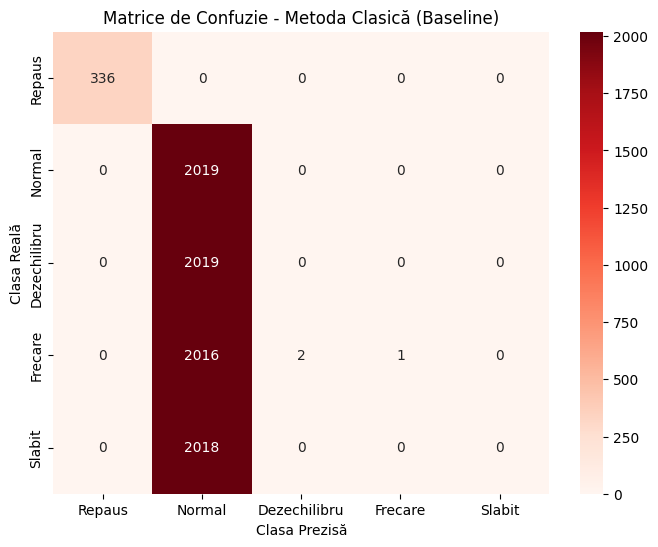
\includegraphics[width=0.45\textwidth]{baseline_cm.png}
		\caption{Matricea de confuzie a sistemului de referință (Baseline). Defectele mecanice sunt clasificate preponderent drept funcționare normală, evidențiind incapacitatea pragurilor euristice de a capta tiparele spațio-temporale complexe.}
		\label{fig:baseline_cm}
	\end{figure}
	
\section{Evaluarea Algoritmilor Clasici}	
	
	
	Algoritmii supervizați Random Forest și Support Vector Machine au avut o acuratețe de aproape 100\%, demonstrând că defectele simulate fizic în mod controlat au o semnătură mecanică distinctă și sunt separabile în noul spațiu al caracteristicilor. Validarea datelor colectate a fost confirmată și de algoritmul nesupervizat K-Means, care a reușit să grupeze corect datele cu o acuratețe de 85\%, deși în faza de antrenament acesta nu a avut acces la etichetele reale.
	
	\begin{figure}[!htbp]
		\centering
		% Prima matrice: Random Forest
		\begin{subfigure}[b]{0.35\textwidth}
			\centering
			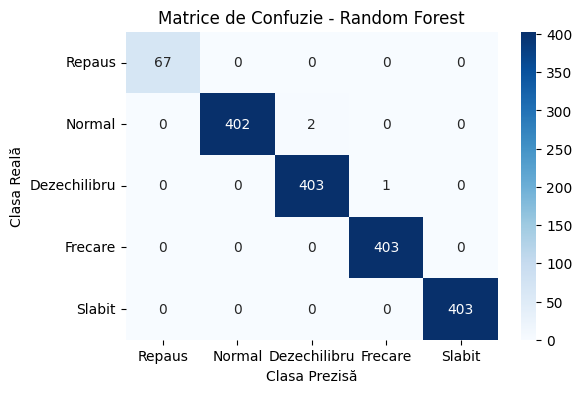
\includegraphics[width=\textwidth]{random_forest_cm.png}
			\caption{Random Forest}
			\label{fig:cm_rf}
		\end{subfigure}
		\hfill
		% A doua matrice: SVM
		\begin{subfigure}[b]{0.35\textwidth}
			\centering
			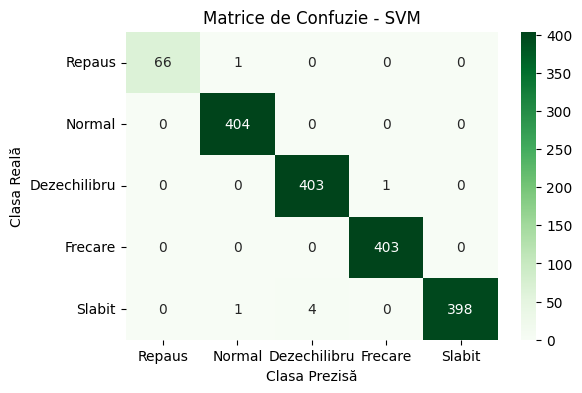
\includegraphics[width=\textwidth]{svm_cm.png}
			\caption{Support Vector Machine (SVM)}
			\label{fig:cm_svm}
		\end{subfigure}
		
		% A treia matrice: K-Means centrată jos
		\begin{subfigure}[b]{0.35\textwidth}
			\centering
			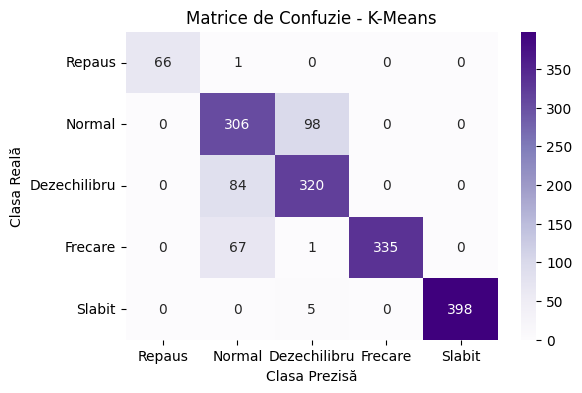
\includegraphics[width=\textwidth]{k_means_cm.png}
			\caption{K-Means Clustering}
			\label{fig:cm_kmeans}
		\end{subfigure}
		\caption{Matricile de confuzie pentru algoritmii clasici evaluați pe spațiul caracteristicilor extrase statistic. Algoritmii supervizați ating performanță aproape perfectă, confirmând separabilitatea claselor; confuziile K-Means apar doar între regimurile active de funcționare.}
		\label{fig:cm_clasici}
	\end{figure} 
	
	Matricile de confuzie din Figura \ref{fig:cm_clasici} confirmă performanța foarte bună a algoritmilor supervizați în clasificarea defectelor. În cazul K-Means, confuziile apar strict în regimul de funcționare Normal, Dezechilibru și Frecare, în timp ce stările de Repaus și Fixare slabă sunt identificate corect majoritatea cazurilor.
	
\section{Arhitecturile Convoluționale}
	
	Cele trei arhitecturi convoluționale evaluate — CNN 1D, CNN 2D și CNN 3D — au obținut acurateți de validare ridicate, de peste 90\%. Modelul CNN 1D, selectat pentru implementarea pe microcontroler, a atins o acuratețe de validare de peste 99,9\% în doar 30 de epoci. Matricile de confuzie corespunzătoare sunt prezentate în Figura~\ref{fig:cnn_cm}.
	
	
	\begin{figure}[!htbp]
		\centering
		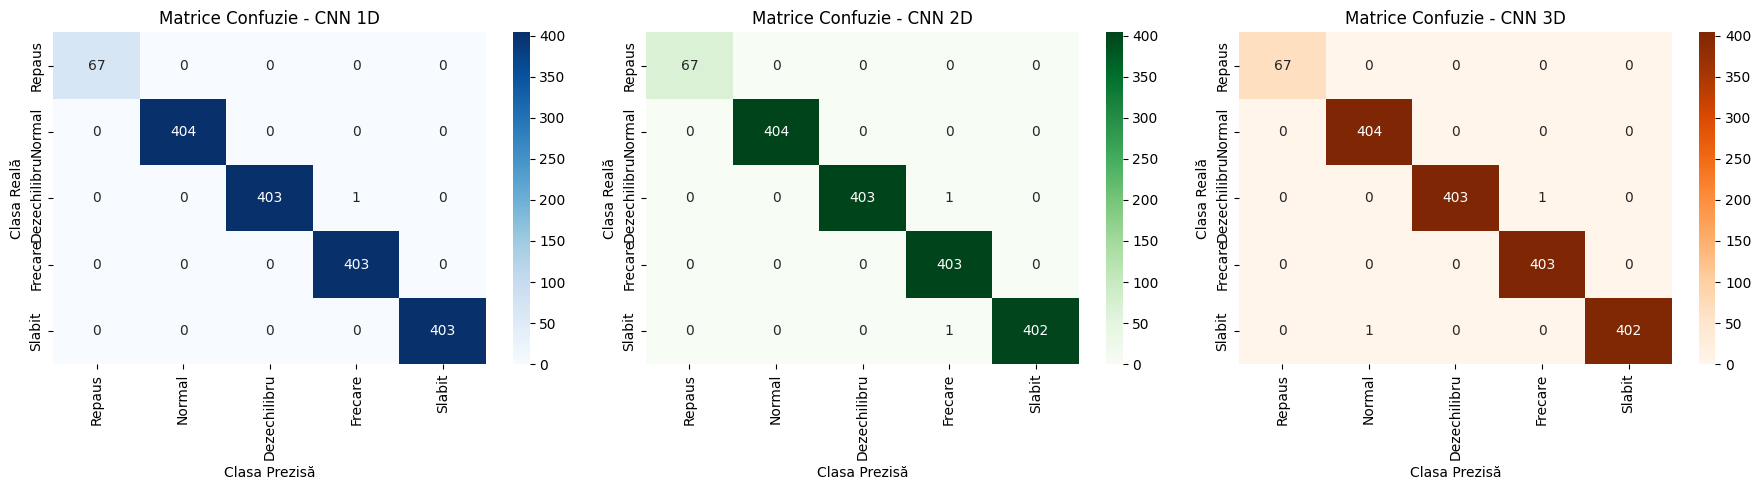
\includegraphics[width=1\textwidth]{cnn_cm.png}
		\caption{Matricile de confuzie ale celor trei arhitecturi convoluționale. Toate depășesc 99\% acuratețe de validare, însă doar CNN 1D are amprenta computațională adecvată implementării pe microcontroler.}
		\label{fig:cnn_cm}
	\end{figure}
	
\section{Compromisul TinyML: Feature Engineering vs. End-to-End Learning}
	
	Modelele clasice sunt rapide la inferență și consumă mai puțină memorie decât rețeaua convoluțională. Deși extragerea caracteristicilor trebuie implementată manual în C++ pe microcontroler, aceasta nu reprezintă un cost semnificativ: pentru implementarea pe dispozitiv am păstrat doar cele trei caracteristici cele mai ieftine de calculat (Media, Deviația Standard și RMS), și am renunțat la Skewness și Kurtosis. Astfel, Random Forest a obținut cel mai mic timp de inferență pe ESP32 (2,56 ms), incluzând extragerea caracteristicilor. Avantajul rețelei convoluționale nu constă în viteză, ci în faptul că învață singură caracteristicile direct din cele 768 de eșantioane brute, eliminând nevoia de a le proiecta și implementa manual la costul unui timp de inferență mai mare (96 ms) și al unei memorii suplimentare ($\sim$35 KB RAM).
	
	\begin{table}[htbp]
		\centering
		\caption{Comparație între modelele evaluate: acuratețe, timp de inferență pe ESP32 și amprentă de memorie. Random Forest oferă cea mai rapidă inferență (2,56 ms), însă CNN 1D este singurul model care rulează stabil pe dispozitiv fără post-procesarea predicțiilor de defect.}
		\label{tab:comparatie}
		\resizebox{\textwidth}{!}{%
			\begin{tabular}{lcccp{3.2cm}}
				\hline
				\textbf{Model} & \textbf{Acuratețe} & \textbf{Timp inf.} & \textbf{Memorie} & \textbf{Observații pe device} \\
				\hline
				Baseline (euristic) & 28\%      & $\sim$0  & neglijabil & -- \\
				Random Forest       & $\sim$100\% & 2,56 ms & redusă & necesită filtru de vot majoritar \\
				SVM (liniar)        & $\sim$100\% & neportat & redusă & -- \\
				K-Means             & 85\%      & neportat & redusă & -- \\
				CNN 1D              & >99,9\%   & 96 ms    & 11,5 KB Flash + 35 KB RAM & stabil; regulă auxiliară pentru Repaus \\
				\hline
			\end{tabular}%
		}
	\end{table}
	
	În testele fizice pe ESP32 \cite{esp32_datasheet}, Random Forestul fără implementarea de filtru de vot majoritar prezicea aproape constant starea de Dezechilibru. CNN1D nu a avut această problemă, însă a necesitat o regulă auxiliară pentru clasa Repaus implementată pe giroscop datorită subreprezentării acesteia în setul de date. Timpii de inferență măsurați pe ESP32 \cite{esp32_datasheet} sunt 2,56 ms pentru Random Forest, respectiv 96 ms pentru CNN1D, ambii suficienți pentru predicții în timp real.
	
	
	Pe când abordarea cu rețeaua convoluțională mută complexitatea preprocesării datelor în arhitectura rețelei. Rețeaua convoluțională are abilitatea de a analiza direct cele 768 de eșantioane brute, deoarece filtrele convoluționale învață singure să extragă caracteristicile specifice spațio-temporale. Astfel, sistemul ales de mine spre implementare reduce necesitatea computațională pentru preprocesare, deși este dependent de framework-ul TensorFlow Lite Micro \cite{tensorflow:tflitemicro_github}, care a fost implementat prin portul TensorFlowLite\_ESP32 \cite{tanaka2026tflite_esp32}, și necesită alocarea unei memorii mai mari, aproximativ 35 KB RAM de tip Tensor Arena. \cite{tensorflow:tflitemicro_github}
	
	